%chapters/result.tex
\subsection{Performance of Sparse Reconstruction}
This paper uses Matlab to evaluate the performance of the proposed system. In the simulation, the UWB waveform is a periodic simple pulse which is shaped by the second derivative Gaussian wave with a pulse duration of 1ns. The bandwidth of this signal is 8GHz. The UWB channel model is based on the IEEE 802.15.4a CM1 model for line of sight (LOS) indoor environment, and zero-mean additive white Gaussian noise (AWGN) is added to generate an average SNR of 10dB. The simulation results cover random points in an area of 10m $\times$ 10m $\times$ 10m space.

The Fig.\ref{res1} demonstrates the TOA estimation average error under different sampling rates. The received signal can be recovered from a certain amount of CS measurements $M$ which is far less than $N$ (Nyquist rate), where compression ratio (CR) equals $\lfloor{M/N}$. In the simulation, three types of different UWB positioning system are tesed: 1) CS Receivers for UWB positioning (CSRD), where random demodulator is implemented at receivers, and the CR refers to the sampling rate of its ADC. 2) The CS pre-coding transmitter (CSPC), where Nyquist rate random projection is implemented at transmitters and downsampling is realized at its receivers. The CR refers to the downsampling rate at its receivers. 3) The proposed new architecture, low-rate CS pre-mixing (LRCSPM) for UWB positioning system, where sub-Nyquist rate random projection is implemented at transmitters and downsampling is realized at its receivers. In this new system, CR refers to the downsampling rate at its receivers, and especially, the low-rate pre-filtering is accomplished by mixing a pseudo-random sequence (PRS) which alternates at a (CR + 10\%) of Nyquist rate.  

\subsection{Performance of CS based Positioning System}
As shown in Fig.\ref{res1}, when the Sampling rate comes close to ???, the average error of all CS-based UWB system has been converges to less than 10mm. However, when the compression ratio continuously increases, the error converging speed of LRCSPM cannot catch up with the speed of others. This is because that if we manage to reduce the highest rate at transmitters in LRCSPM, as a result, the required sampling rate must be increased as a sacrifice at receivers, otherwise the estimation error rate will increase. Furthermore, if we increase the sub-Nyquist sampling rate  by 10\% of CR at receivers, which creates a revised system named LSCSPF-R, then it produce outstanding performance: when compression ratio becomes less than 0.15 and continuously decreases, the advantage of the proposed LRCSPM emerges: the error increasing speed is far slower than the others. This result suggests that the LSCSPF-R (the revised low-rate CS pre-mixing system) outperforms the traditional CS UWB positioning systems in terms of estimation error at lower compression ratio. 

Besides, the CSRD, CSPC, and LSCSPF all provide sub-mm estimation error with enough CS observations (CR $>$ 0.15), while the original UWB TOA system contains an average error around 3.92mm. Thus, CS UWB TOA positioning system can achieve a much higher positioning accuracy than the traditional system. 

Therefore, the simulation result shows that the proposed system (LSCSPF) successfully improves the positioning error compared to original system. The results also demonstrates that the system trade-off among random projection rate, sub-Nyquist sampling rate and estimation error: 1) if the downsampling rate at receivers keeps the same, the average error increases at mm level. In addition, if CR $>$ 0.15, then the increased error will be constrained to be less than 1mm, which is relatively small and almost can be neglected. 2) if we want to catch up with the performance of the average error compared to that in other two CS UWB systems (CSRD and CSPC), we need to increase the compression ratio (CR) by nearly 10\% (shown in the curve of LSCSPF-R). Notice it is worthy because even if we add 10\% of CR to the clock rate of sampling at receivers, the CR still remains relatively low (around 0.25 in many cases) for ADCs, correspondingly equals only 1/4 sub-Nyquist rate.     

\begin{figure}[!t]
\centering
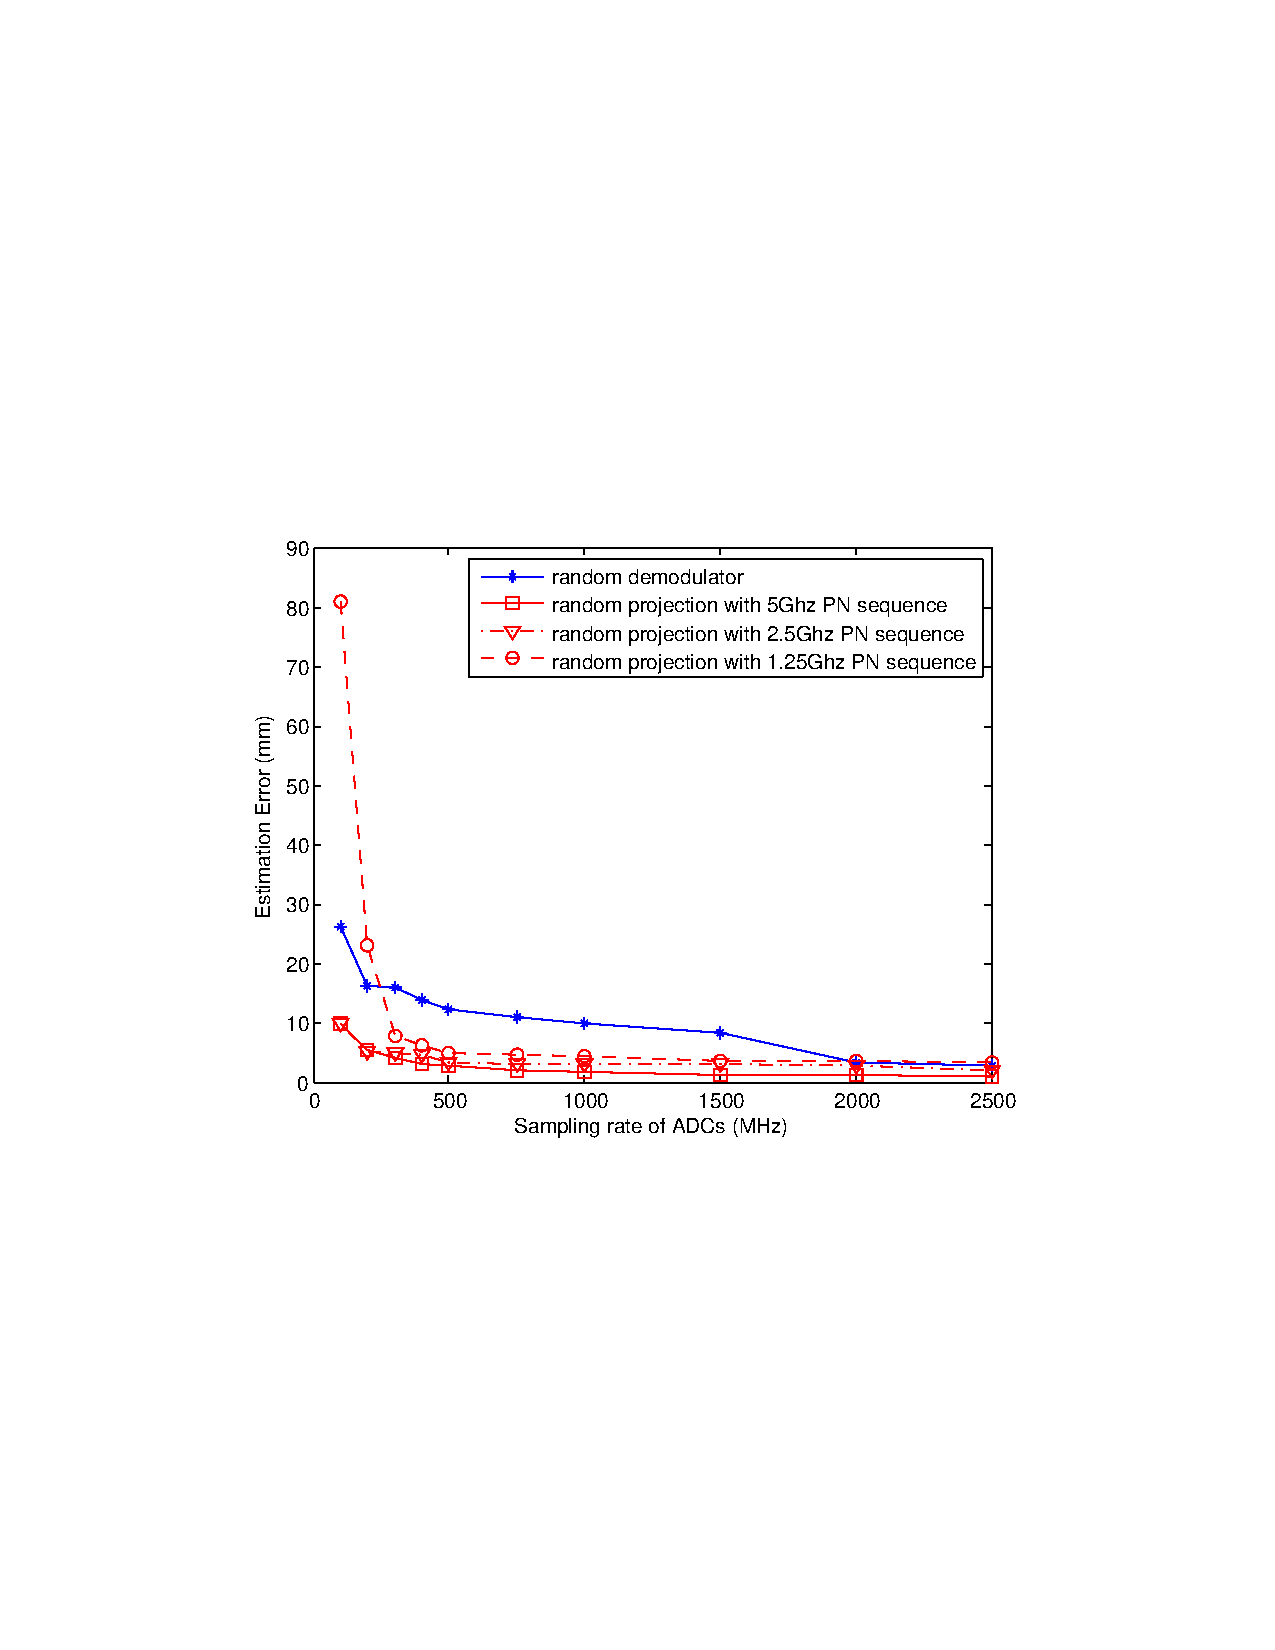
\includegraphics[width=3.2in]{res1.pdf}
\DeclareGraphicsExtensions.
\caption{CS based TOA estimation average error under different compression ratio based on the IEEE 802.15.4a CM1 model for line of sight (LOS) indoor environment}
\label{res1}
\end{figure}
